\documentclass{standalone}
\usepackage{tikz}
\usepackage{amsmath}

\begin{document}
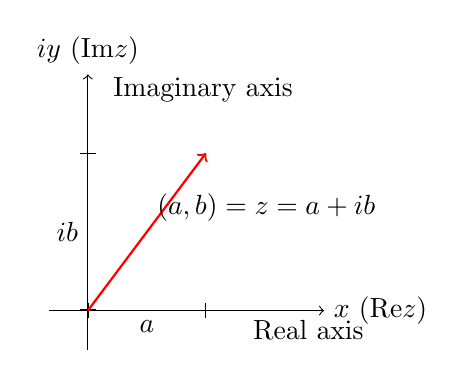
\begin{tikzpicture}[scale=1] %Adjust scale as needed
  % Axes
  \draw[->] (-0.5,0) -- (3,0) node[right] {$x$ (Re$z$)};
    \node[below] at (2.8,0) {Real axis};
  \draw[->] (0,-0.5) -- (0,3) node[above] {$iy$ (Im$z$)};
    \node[right] at (0.2, 2.8) {Imaginary axis};

  % Point a on the real axis
  \draw[|-|] (0,0) -- (1.5,0) node[midway, below] {$a$};

  % Point ib on the imaginary axis
  \draw[|-|] (0,0) -- (0,2) node[midway, left] {$ib$};

  % Vector representing z = a + ib
  \draw[->, red, thick] (0,0) -- (1.5,2) node[midway, above right, black] {$(a,b) = z = a + ib$};

\end{tikzpicture}
\end{document}